\chapter{Introducción}

Los sistemas embebidos son aquellos sistemas de hardware y software optimizados para
implementar una función específica. Los criterios de optimización
suelen enfocarse en reducir el costo, el consumo y el tamaño. Los
problemas que pueden resolverse mediante tales sistemas van desde un
simple control de temperatura para un acondicionador de aire hasta el
sistema de control y el procesamiento de señales en un satélite de
telecomunicaciones. La gran eficiencia que han demostrado los sistemas
embebidos en la solución de problemas específicos ha producido un
incremento significativo en su demanda. En particular, actualmente se
quiere expandir la capacidad de los mismos para atacar problemas de
mayor complejidad y reducir los tiempos de desarrollo ofreciendo una
más rápida puesta en funcionamiento. Esto último en particular es de
gran importancia a nivel competitivo ya que la rápida evolución de la
tecnología hace que un tiempo de desarrollo prolongado tenga como
consecuencia un producto basado en una tecnología parcialmente
obsoleta.

\section{Motivación}

Para reducir los costos y el tiempo de desarrollo, el diseño de
sistemas embebidos utiliza como base una plataforma hardware sobre la
que se pueden construir un amplio número de aplicaciones. Esta
flexibilidad en las aplicaciones soportadas es posible debido
a que tales plataformas disponen de múltiples puertos capaces de
manejar señales de diferentes tipos. Las plataformas más comunes
actualmente son los microcontroladores (MCUs) y los procesadores
digitales de señal (DSPs). Con dichas plataformas, el diseño de la
aplicación consiste, primordialmente, en el desarrollo del software
asociado a la misma. Por tal motivo, los fabricantes de dichas
plataformas, habiendo ``solucionado'' el problema del hardware, comenzaron a proveer soluciones para el software asociado. En particular, las nuevas series de MCUs soportan sistemas
operativos, lo que facilita significativamente el desarrollo de las
aplicaciones que va a soportar el sistema final. Sin embargo, a pesar
de las grandes ventajas de disponer de soluciones listas tanto para
el hardware como para el software, existe una contrapartida que radica
en el hecho de que son plataformas estáticas. Esto último hace casi
imposible realizar un diseño que esté realmente optimizado para la
aplicación que nos interesa.

Una alternativa a las plataformas de hardware estáticas se basa en la
utilización de en inglés Field Programmable Gate Array (FPGAs). La alta capacidad de integración, el bajo coste
para la fabricación de pequeños lotes y el alto rendimiento, en
términos de frecuencia de operación y consumo de potencia, hacen
posible implementar un SoC en este tipo de dispositivo
programable. Los SoC que se pueden implementar sobre las FPGAs tienen
una serie de ventajas sobre las plataformas estáticas, como la
adaptación a cualquier necesidad específica o la reconfiguración
dinámica. Sin embargo, el uso de FPGAs implica necesariamente un
esfuerzo para diseñar la arquitectura hardware que, evidentemente,
incrementa el tiempo de desarrollo total del sistema.

Para que el diseño de sistemas embebidos basados en FPGAs sea
competitivo frente a los sistemas basados en MCU o DSP, es necesario
facilitar la construcción de la arquitectura hardware. En particular,
se debe disponer de metodologías de diseño eficientes basadas en
herramientas CAD adecuadas a tal fin. Por tal motivo, el principal
esfuerzo que están haciendo los fabricantes de FPGA está dirigido a
mejorar las herramientas de diseño 
de hardware sobre FPGAs. En este sentido
existe un alto nivel de competitividad para encontrar la solución que
provea simultáneamente una gran simplicidad en el diseño de la
arquitectura hardware y un alto rendimiento del sistema
final. Ejemplos de estas herramientas son Xilinx EDK y Altera ESD. Sin
embargo, lo anterior no es suficiente para lograr la competitividad de
los sistema embebidos basados en FPGAs. Es necesario también
simplificar el desarrollo del software asociado a los mismos, en
particular teniendo en cuenta que los MCU ya soportan sistemas
operativos completos. Los SoC sobre FPGAs recientemente empiezan a
tener soporte para sistemas operativos tales como Petalinux
MicroBlaze, o proyectos de portar Linux a Nios o a Lattice
Mico32. Desafortunadamente, tales soluciones son nuevamente
privativas.

Lo anterior llega nuevamente a la necesidad de explorar el diseño de
SoC sobre FPGAs utilizando sistemas abiertos tanto a nivel de hardware
como de software. Tales sistemas abiertos se caracterizan porque son
tecnológicamente independientes y pueden implementarse tanto a
nivel de FPGAs de bajo coste como a nivel de Circuito Integrado para Aplicaciones Específicas (ASIC). Existen softcores
de código abierto que no están limitados por la tecnología. Entre
dichos núcleos, se destacan los microprocesadores de 32 bits
\textit{SPARC LEON, OpenRISC 1200} y \textit{LatticeMico32}.

Las premisas que propone la Free Software Foundation (FSF) al usar cores de código abierto va unido a una serie de conceptos como:
\begin{itemize}
\item \textit{Flexibilidad}: Si el código fuente está disponible, los
  desarrolladores pueden modificar dicho código de acuerdo a sus
  necesidades. Además, se produce un flujo constante de ideas que
  mejoran la calidad del código.
\item \textit{Fiabilidad y seguridad}: Con muchos programadores
  escrutando simultáneamente el mismo trabajo, los errores se detectan
  y corrigen con mayor velocidad, por lo que el producto resultante es
  mas fiable y eficaz que el comercial.
\item \textit{Rapidez de desarrollo}: Las actualizaciones y ajustes se
  realizan a través de una comunicación constante vía Internet.
\item \textit{Relación con el usuario}: El programador se acerca mucho
  más a las necesidades reales de su cliente, y puede crear un
  producto específico para él.
\end{itemize}

La conjunción de dichos conceptos produce un sistema integrale de
código abierto en donde se tiene código HDL, Assembler y C disponible
para adaptarse de acuerdo a los requerimientos del proyecto.


\section{Objetivos}
\subsection{Objetivo general}
El presente proyecto tiene como objetivo la implementación de un sistema embebido basado en hardware\footnote{Entendiéndose por hardware de código abierto al código Register Transfer Level (RTL)} y software de código abierto.
Dicho hardware será un System on Chip (SoC) montado sobre una placa de desarrollo que deberá además soportar un sistema operativo
libre con la finalidad de proveer un sistema integral FPGA-SoC-Sistema
Operativo completamente funcional de código abierto para aplicaciones de pequeña envergadura.

\subsection{Objetivos específicos}
  \begin{itemize}
 \item Analizar los microprocesadores softcore disponibles y seleccionar el microprocesador que se adapta mejor a nuestros requerimientos.

\item Seleccionar los SoCs de acuerdo al microprocesador softcore elegido y determinar la placa de desarrollo para su implementación.

\item Implementar el flujo de diseño de hardware para cada SoC seleccionado y realizar las correcciones necesarias sobre el código RTL para su correcta implementación. 
\item Desarrollar  aplicaciones en lenguaje C generadas mediante compilación cruzada para las pruebas del funcionamiento del microprocesador, los SoCs, sus modulos y las herramientas de entorno de software para la arquitectura seleccionada.
\item Estudiar y aplicar los mecanismos para la medición del rendimiento de sistemas embebidos. 
\item Estudiar los Sistemas Operativos existentes soportados por las plataformas elegidas.
\item Presentar los Sistemas Operativos Linux y ecOS que poseen las prestaciones funcionales adecuadas para su utilización en Sistemas Embebidos.
\item Poner en funcionamiento y configurar los sistemas operativos Linux y ecOS para los SoCs elegidos.
 \end{itemize}


\subsection{Alcance de estudio}

El plazo estipulado para el desarrollo del proyecto involucra las siguientes etapas:

\begin{itemize}
\item Especificación y análisis de requerimientos.
\item Análisis de riesgos.
\item Evaluación de componentes.
\item Implementación.
\item Testing.
\end{itemize}

\section{Recursos Utilizados}

La implementación del sistema se llevó a cabo sobre la placa de
desarrollo de Xilinx S3ADSP1800A, basada en hardware reconfigurable disponible en
el Centro Universitario de Automatización y Robótica (CUDAR) de la
Universidad Tecnológica Nacional (UTN) de Córdoba. Sin embargo, cabe
destacar que el sistema propuesto puede ser implementado cualquier
otra FPGA que disponga de los recursos mínimos necesarios.

\section{Modelo de Desarrollo}
El modelo de desarrollo a utilizar es el \textit{Modelo en
  Espiral} figura~\ref{fig:pepe}. Dicho modelo fue tipificado por Ian
Sommerville~\cite{Etiqueta00} y originalmente propuesto por Boehm en
año 1988 en el artículo ``A Spiral Model of Software Development and
Enhancement''. En el mismo se propone un marco del proceso de software
dirigido por el riesgo. Aquí, el proceso de desarrollo se representa
como una espiral en donde cada ciclo en la espiral representa una fase
del proceso de desarrollo. Por ende, el ciclo más interno puede
relacionarse con la factibilidad del sistema, el siguiente ciclo con
la definición de requerimientos, el siguiente ciclo al diseño del
sistema, y así sucesivamente.

\begin{figure}[h!]
 \begin{center}
  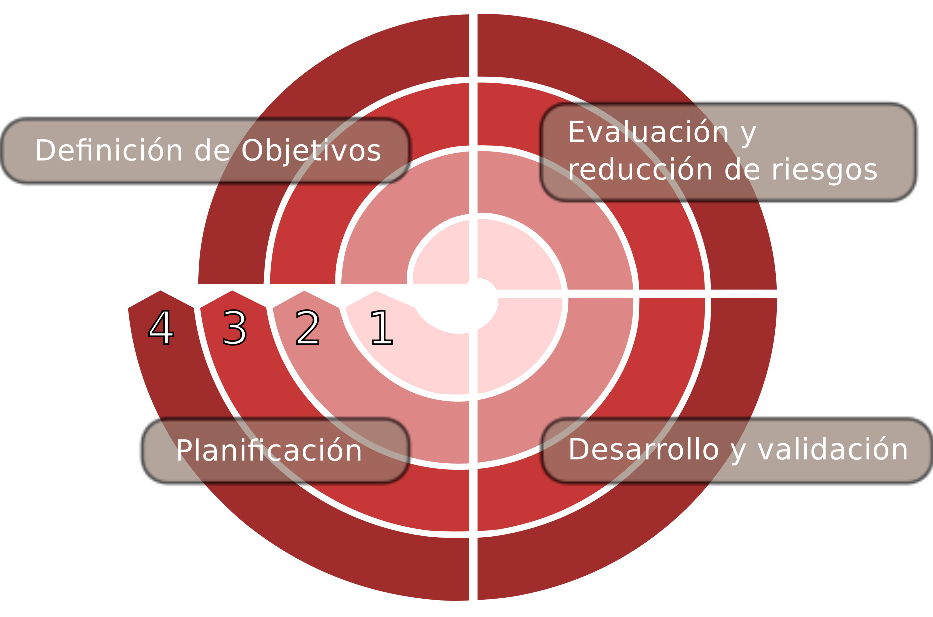
\includegraphics[width=1\textwidth,keepaspectratio=true]{./images/espiral.pdf}
  \caption{Etapas del modelo de desarrollo en espiral}
  \label{fig:pepe}
 \end{center}
\end{figure}

Cada ciclo del espiral se divide en 4 sectores:
\begin {itemize}
\item \textit{Establecimiento de objetivo}: Se definen objetivos
  específicos para dicha fase del proyecto. Se identifican
  restricciones en el proceso y en el producto y se traza un plan
  detallado de gestión. Se identifican los riesgos y se planean
  estrategias que brinden caminos alternativos hacia la solución como
  respaldo en caso de la aparición de problemas asociados a los
  riesgos identificados.
\item \textit{Validación y reducción del riesgo}: En cada uno de los
  riesgos identificados del proyecto, se realiza un análisis
  minucioso proponiendo acciones para reducir dichos riesgos.
\item \textit{Desarrollo y validación}: Después de una evaluación de
  riesgos, se elige un modelo de desarrollo para el sistema.
\item \textit{Planeamiento}: El proyecto se revisa y se toma una
  decisión sobre si hay que continuar con otro ciclo de la espiral. Si
  se opta por continuar, se trazan los planes para la siguiente fase
  del proyecto.
\end {itemize}

Como característica principal de esta metodología es que posee una
consideración explícita del riesgo. Informalmente, el riesgo significa
sencillamente que algo puede salir mal. Los riesgos originan problemas
en el proyecto, como los de confección de agendas y excesos en los
costos. Por lo tanto, la disminución de riesgos es una actividad
sumamente importante en la gestión del proyecto. Un ciclo en la
espiral comienza con la elaboración de objetivos, como el rendimiento
y la funcionalidad. Entonces se enumeran formas alternativas de
alcanzar estos objetivos y las restricciones impuestas en cada una de
ellas. Cada alternativa se evalúa contra cada objetivo y se
identifican las fuentes de riesgos del proyecto. El siguiente paso es
resolver estos riesgos mediante actividades de recopilación de
información como la de detallar más el análisis, la construcción de
prototipos y la simulación. Una vez que se han evaluado los riesgos se
llevará a cabo cierto desarrollo, seguido de una actividad de
planificación para la siguiente fase del proceso.

\section{Metodología de Trabajo}

Siendo la primera vez que se plantea un proyecto como el aquí
descripto en el ámbito de la Universidad Nacional de Córdoba, no se
dispone de antecedentes de trabajos similares que involucren
Microprocesadores softcore. Por tal motivo, todo el desarrollo se
realizara desde cero. Como primer paso se analizarán las diferentes
alternativas disponibles en el mercado y en comunidades de hardware de
código abierto para la implementación de microprocesadores diseñados
en lenguaje de descripción de hardware. Como segundo paso 
se analizarán y seleccionarán los componentes \footnote{Entiéndase como ``componente'' a 
microprocesadores softcore, SoC, placa de desarrollo, sistema operativo.} 
por medio de un análisis comparativo que permitirá evidenciar las características relevantes de
cada uno de ellos. Como último paso debido a que se adoptara un modelo de desarrollo en espiral se plantearán una serie de prototipos que incluirán mayor funcionalidad en cada iteración del modelo.


